\documentclass[mathserif]{beamer}

\usetheme{singapore}

\usepackage{graphicx}
\usepackage{tabularx}
\usepackage{longtable}
\usepackage{multicol}
\usepackage{epstopdf}
\usepackage{amssymb}

\title{Saving and Liquidity Constraints}
\author{Angus Deaton}
\institute{Econometrica, Volume 59, No. 5, September, 1991}
\date{4th December, 2015}

\begin{document}
\frame{\titlepage}
\begin{frame}
\frametitle{Key aim of the paper}
\begin{itemize}
    \setlength\itemsep{1em}
    \item This paper is concerned with the theory of optimal intertemporal consumption behaviour who are restricted in their ability to borrow to finance consumption
    \item General rule: Partial equilibrium. Start from a simple stochastic process for labor income. Derive appropriate policy rule/consumption function given borrowing constraint. Study the time-series behaviour of consumption, savings and assets.
\end{itemize}
\end{frame}

\begin{frame}
\frametitle{Roadmap}
\begin{enumerate}
  \item PIH, very briefly
  \item Some empirical evidence
  \item Main results
  \item Basic Model
  \item Some stochastic labor income process, solution, simulations
  \item Repeat 5 with some other stochastic process
\end{enumerate}
\end{frame}

\begin{frame}
\frametitle{The benchmark: Permanent Income Hypothesis}
\begin{itemize}
  \setlength\itemsep{1em}
  \item Assume infinite horizon, stochastic income, quadratic utility, \(\delta = r\) and no borrowing constraints
  \item We get: Consumption is a random-walk (Hall, 1978), depends only on annuity value of income. Consumption will only change when new/unanticipated information about permanent income is revealed
  \item Also, certainty equivalence: variance and higher moments of the income process do not matter for the determination of consumption
\end{itemize}
\end{frame}

\begin{frame}
\frametitle{Empirical evidence, 1}
\begin{itemize}
  \setlength\itemsep{1em}
  \item Campbell and Deaton (1989): Assume aggregate income process: \(\Delta y_{t} = \lambda \Delta y_{t-1} + \epsilon_{t}\) 
  \item Apply it to the PIH model
  \item For plausible values of $r$ and $\lambda$ they found that permanent income (current consumption) can be twice as variable as current income. Data showed consumption is less variable than (current) income $\rightarrow$ Deaton's paradox (excessive smoothness of aggregate consumption, relative to PIH/LC)
\end{itemize}
\end{frame}

\begin{frame}
\frametitle{Empirical evidence, 2}
\begin{itemize}
  \setlength\itemsep{1em}
  \item Consumption is a random walk, cannot be predicted from past information
  \item Flavin (1981) and many subsequent authors: changes in consumption are positively relate to predictable changes in income
  \item Furthermore, Carroll and Summers (1989)  show that consumption appears to track household income quite closely over life cycle
  \item Moreover, most versions of the life-cycle models predict a dissociation of consumption from income, and the existence of substantial asset at least at some points in the life-cycle. 
      \begin{itemize}
        \item Validity challenged. Most US household's hold very few assets, estimates vary but median household wealth, excluding pension
      \end{itemize}
  \end{itemize}
\end{frame}

\begin{frame}
\frametitle{Towards borrowing constraints (and impatience)}
\begin{itemize}
  \setlength\itemsep{1em}
  \item In summary, existing empirical evidence at the time showed consumption responds to predictable change in income $\rightarrow$ Euler equation violated
  \item Many households have little financial wealth, unlikely to be able to finance consumption by borrowing
  \item Large share of consumers do not have many financial assets despite strong savings incentives $\rightarrow$ households may be less patient than when \(\delta = r\)
\end{itemize}
\end{frame}

\begin{frame}
\frametitle{Main results, 1}
\begin{itemize}
  \setlength\itemsep{1em}
  \item Impatience + BC + prudence $\rightarrow$ behaviour of saving and accumulation quite sensitive to stochastic process generating income
  \item Stationary, i.i.d income: asset are buffer stock, consumers save and dissaves to smooth consumption (smoother than income), more prudent consumer + more uncertain income = more precautionary balance
  \item Positive serial correlation: desirability and feasibility of using assets as buffer diminishes.
  \item Random walk: consume all your income
\end{itemize}
\end{frame}

\begin{frame}
\frametitle{Main results, 2}
\begin{itemize}
  \setlength\itemsep{1em}
  \item Stationary income growth, growth mimics aggregate data: paradoxical result, savings is counter-cyclical
  \item Agent's income process independent, with negative serial correlation in growth rates: No savings in the aggregate
  \item Combination of aggregate and idiosyncratic income process: generates savings in the aggregate, can potentially reproduce stylized facts in the actual data
\end{itemize}
\end{frame}

\begin{frame}
\frametitle{Basic model}
Standard intertemporal utility maximization. Consumer receives \(y_{t}\), stochastic. Given $r$. \\\

Assumptions: 
\begin{enumerate}
  \item BC: \(A_{t} \geq 0\)
  \item Prudence: \(u''' \geq 0\)
  \item Impatience: \(\delta \geq r\)
\end{enumerate}
\end{frame}

\begin{frame}
\frametitle{Case 1: i.i.d. income shock}

Suppose \(y_{t}\) is i.i.d with distribution $F(\centerdot)$. No persistence, no growth. Relaxed later.

\begin{equation}\label{1}
  u = E_{t}(\sum_{\tau = t}^{\infty}(1+\delta)^{t-\tau}\upsilon(c_{\tau}))
\end{equation}

\begin{equation}\label{2}
 \text{s.t.}\quad A_{t+1} = (1+r)(A_{t} + y_{t} - c_{t})
\end{equation}
\end{frame}

\begin{frame}
\frametitle{The Euler Equation}
Define, $x_{t}$ as "cash on hands" as \(x_{t} = A_{t} + y_{t}\) \\\

Hence, 
\begin{equation}\label{4}
 \lambda(c_{t}) = max[\lambda(x_{t}), \beta E_{t} \lambda(c_{t+1})]
\end{equation}

\begin{equation*}
\text{where}\quad\lambda(c_{t}) = \upsilon'(c_{t})
\end{equation*}
\end{frame}


\begin{frame}
\frametitle{Solution methods}
\begin{enumerate}
  \setlength\itemsep{1em}
  \item Solve simultaneously the two difference equations in Eq.(2) and Eq.(3)
  \item Alternatively, work through the following value function
    \begin{equation}
        V(x) = \underset{0 \leq s \leq x}{\max}\Bigg\{\upsilon(x-s) + (1+\delta)^{-1}\int V[(1+r)s + y] dF(y )\Bigg\}
    \end{equation}  
\end{enumerate}   
\end{frame}

\begin{frame}
\frametitle{Solution, 1: Buffer-stock behaviour}
\begin{equation*}
  c = f(x) = x, \quad x\leq x^{*}
\end{equation*}

\begin{equation*}
  c = f(x) \leq x, \quad x\geq x^{*}
\end{equation*}

\begin{enumerate}
  \item If total income below the critical level, everything is spent, and the household goes into the next period with no assets. If the total is greater that \(x^{*}\), something will be held, positive level of assets carried forward
  \item Assets are not desired for their own sake, but to buffer fluctuations in income. High income, saving. Low income, dissaving
  \item Distribution of consumption not symmetric
\end{enumerate}
\end{frame}


\begin{frame}
\frametitle{Solution, 2}
\begin{figure}
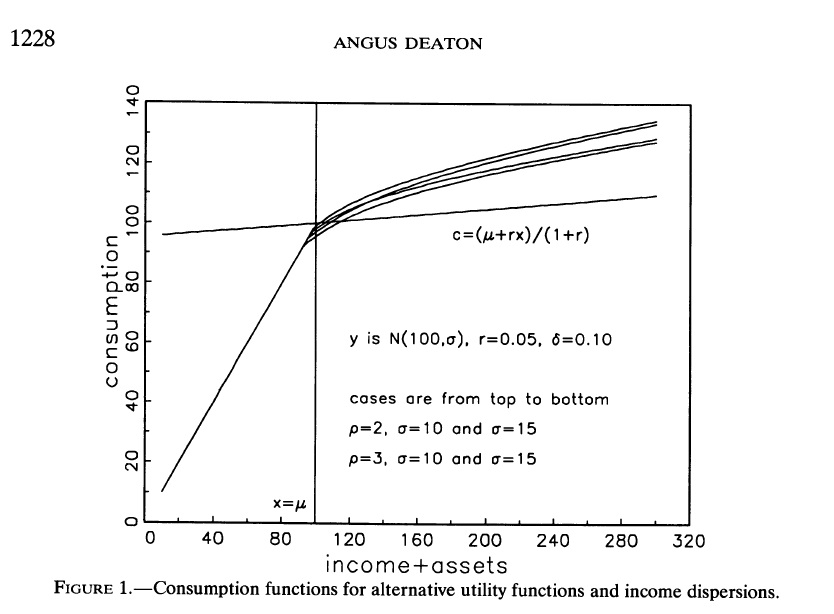
\includegraphics[height=2.5 in, scale=0.5]{figure1.jpg}
\end{figure}
\end{frame}

\begin{frame}
\frametitle{Simulation}
\begin{figure}
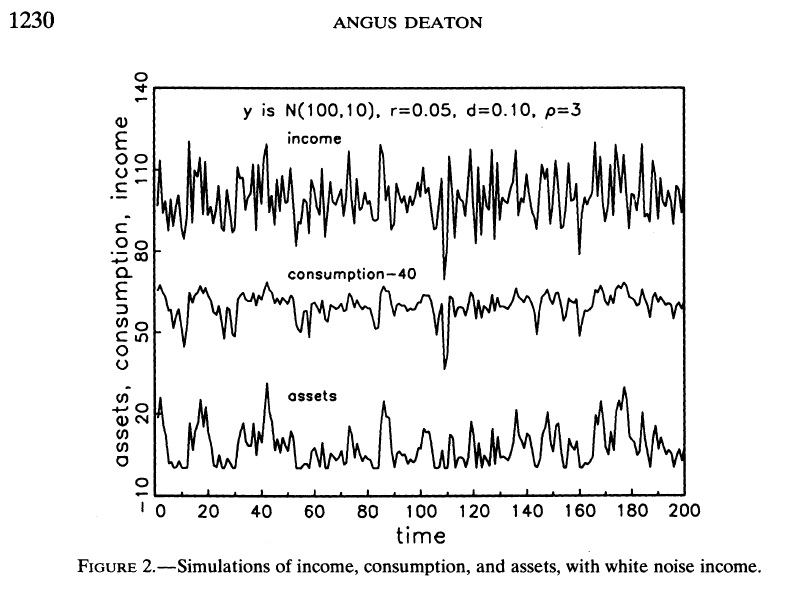
\includegraphics[height=2.5 in, scale=0.5]{figure2.jpg}
\end{figure}
\begin{enumerate}
  \item 200 period simulation, consumption notably smoother
  \item However, depends on sd of income and prudence though
\end{enumerate}
\end{frame}

\begin{frame}
\frametitle{Case 2: Stationary serially correlated income}

Is i.i.d. a reasonable assumption?
Maybe for farmers in LDC's whose income depends on weather. Even for them, many behavioural and technical responses are likely to generate correlated income processes. For advanced countries? maybe, not \\\

Towards serially correlated income \\\

\end{frame}

\begin{frame}
\frametitle{Value function}

Assume, income follows AR(1).  

\begin{equation*}
    (y_{t} - \mu) = \phi(y_{t - 1} - \mu) + \epsilon_{t}
\end{equation*}

Essentially, the same problem. But, with two state variables. Cash in hand today and income today used to predict expected marginal utility of consumption tomorrow.

\begin{equation}
        V(x, y^{cur}) = \underset{0 \leq s \leq x}{\max}\Bigg\{\upsilon(x-s) + (1+\delta)^{-1}\int V[(1+r)s + y] dF(y | y^{cur})\Bigg\}
\end{equation}
\end{frame}

\begin{frame}
\frametitle{Solution: same buffer-stock behaviour}
\begin{figure}
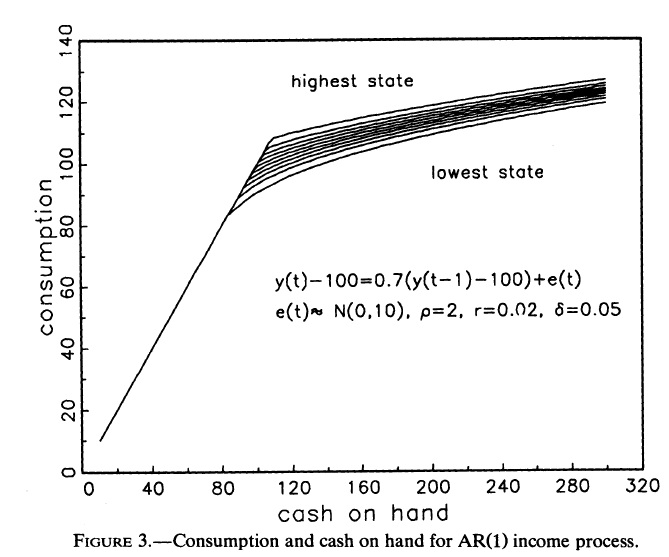
\includegraphics[height=2.5 in, scale=0.5]{figure3.jpg}
\end{figure}
\end{frame}

\begin{frame}
\frametitle{Simulation, 1}
\begin{figure}
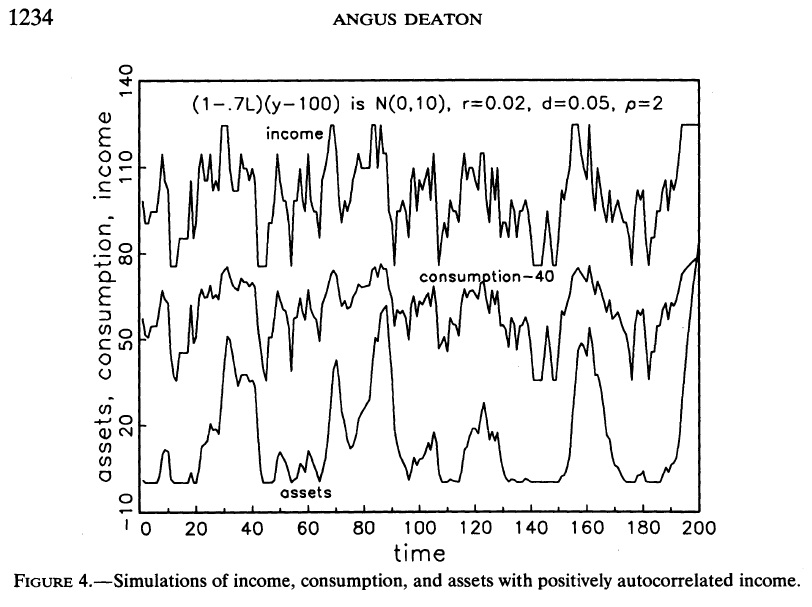
\includegraphics[height=2.5 in, scale=0.5]{figure4.jpg}
\end{figure}
\end{frame}

\begin{frame}
\frametitle{Simulation, 2}
    \begin{enumerate}
      \item Consumption again smoother than income, but less so. Sd(c) is 10.4, sd(y) is 14
      \item Savings pro-cyclical, large assets are occasionally accumulated. 
      \item Quite long periods of no or close to zero assets, more likely the more positively autocorrelated is income
      \item Asymmetric behaviour of consumption still prominent
    \end{enumerate}
\end{frame}

\begin{frame}
\frametitle{Simlation, 3}
\begin{figure}
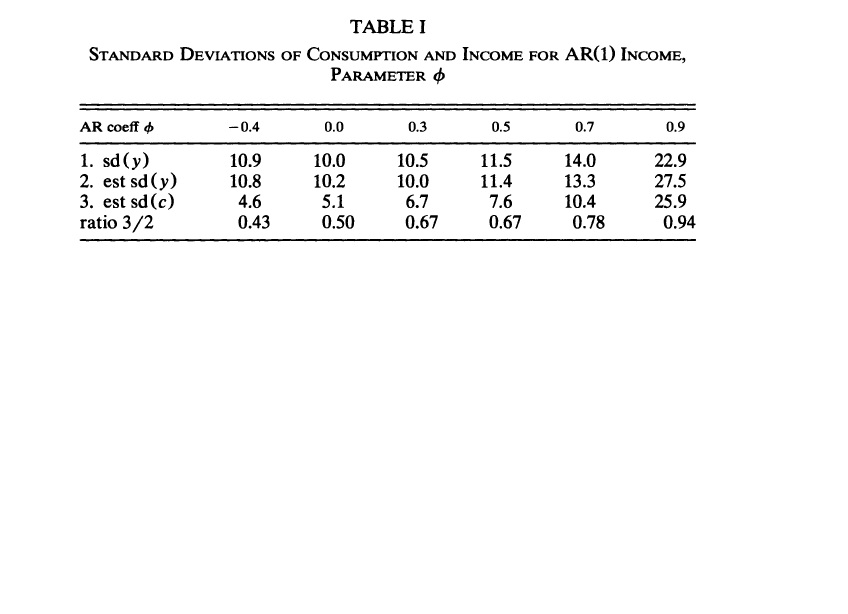
\includegraphics[height=2.5 in, scale = 0.5]{table1.jpg}
\end{figure}
\end{frame}

\begin{frame}
\frametitle{Continue}
\begin{enumerate}
  \item For the i.i.d. case, optimal smoothing can remove half of the standard deviation of income, but as autocorrelation increases consumption becomes as noisy as income
  \item Impatient consumers. Precautionary demand powerful motive for assets, but smoothing consumption over long autocorrelated swings require more consumption sacrifice.
\end{enumerate}
\end{frame}

\begin{frame}
\frametitle{Case 3: Random walks,1}
However, most consumers in developed and developing economies can reasonably expect income to grow over time. If such expectations are held, analysis will be very different 

\begin{itemize}
  \item  With income growth implications are different. For agents with \(\delta > r\), individuals more likely to be liquidity constraint
  \item Assume isoelastic preferences with relative risk aversion parameter $\rho$
  \item Assume no uncertainty, no initial assets. Consumption should grow at rate \(\rho^{-1} (r-g)\)
  \item If income grows at \(g > \rho^{-1} (r-g)\) $\rightarrow$ borrowing will be required, more likely to be income constrained
\end{itemize}
\end{frame}

\begin{frame}
\frametitle{Case 3: Random walks, 2}
\begin{enumerate}
  \item Logarithm of the income process is stationary in first-differences
  \item Such models capable of modelling actual aggregate household income in the U.S.
\end{enumerate}
\end{frame}

\begin{frame}
\frametitle{Model}

\begin{itemize}
  \item Same problem as before but log od income follows a random walk. Assume isoelastic preferences
\end{itemize}

\begin{equation*}
 z_{t+1} = \frac{y_{t+1}}{y_{t}}
\end{equation*}

\begin{equation*}
    \lambda(\theta_{t}) = max[\lambda(_{t}), \beta E_{t} z_{t+1}^{\rho} \lambda(\theta_{t+1})]
\end{equation*}

where \(\theta_{t} = \frac{c_{t}}{y_{t}}\) and \(w_{t} = \frac{x_{t}}{y_{t}}\)

\begin{equation*}
 w_{t+1}=1+(1+r)(w_{t} + \theta_{t}) z_{t+1}^{-1}
\end{equation*}
\end{frame}

\begin{frame}
\frametitle{Value function and intuition}
\begin{equation}
        V(w) = \underset{0 \leq \theta_{t} \leq x}{\max}\Bigg\{\upsilon(\theta_{t}) + (1+\delta)^{-1}\int V[1+(1+r)(w + \theta) z^{-1}] dF(z)\Bigg\}
\end{equation}

\begin{itemize}
  \item With random walk we get the result that consumption is equal to income
  \item Presence of binding constraints makes it undesirable to undertake smoothing
  \item Suppose consumer has no asset, income growth well above average
  \item May seem like a good situation to save, but consumer is already liquidity constrained
\end{itemize}
\end{frame}

\begin{frame}
\frametitle{Continue}

\begin{itemize}
    \item Additional income merely provides an opportunity to get closer to the ideal consumption path which would have been the case when no BC $\rightarrow$ good draws in income are spent, assets remain at zero
  \item But, saving is desirable when income is expected to be lower?
  \item However, RW implies that while a bad draw does indeed imply that income thereafter can expected to be permanently lower, expected growth rate of income is unchanged
  \item There is never any rational expectation that income will be lower
\end{itemize}
\end{frame}

\begin{frame}
\frametitle{Case 4: Autocorrelated growth rates}
\begin{itemize}
  \item Post war US quarterly data, the growth of aggregate hh income better approximated by AR(1)
  \item For both GDP and income, growth shocks are persistent, positive shocks followed by positive shocks
  \item Incorporating such an income process is capable of generating some savings, even in the presence of BC, but don't behave in the same way as aggregate data
\end{itemize}
\end{frame}

\begin{frame}
\frametitle{Model}
\begin{itemize}
  \item Take the same setup as in Case 3  
  \item Two state Markov process with noise, keeps calculations simple
  \item State 1 = "boom", State 2 = "slump"
\end{itemize}
\begin{equation*}
  \text{when state 1}\quad\Delta \ln y_{t} = g_{1} + \epsilon_{t}
\end{equation*}

\begin{equation*}
  \text{when state 2}\quad\Delta \ln y_{t} = g_{2} + \epsilon_{t}
\end{equation*}

where \(g_{2} < 0 < g_{1}\) and \(\epsilon_{t}\) is a gaussian white noise.\\\


Transition probabilities are \(\psi_{1} = pr(s_{t} = 1 | s_{t-1} = 1)\) and \(\psi_{2} = pr(s_{t} = 2 | s_{t-1} = 2)\). Economy shows positive growth on average \((1 - \psi_{2})g_{1} + (1 - \psi_{1})g_{2} > 0\)

\end{frame}

\begin{frame}
\frametitle{Solution}
\begin{figure}
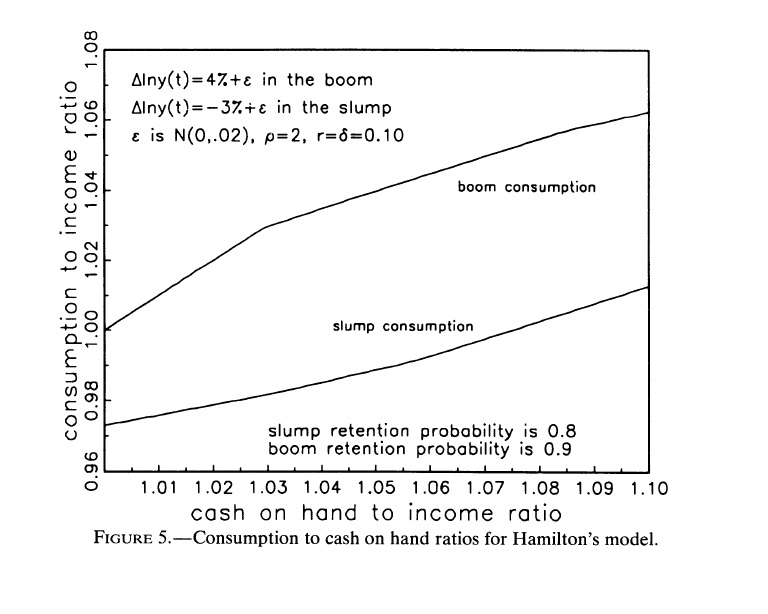
\includegraphics[height=2.5 in, scale=0.5]{figure5.jpg}
\end{figure}
\end{frame}

\begin{frame}
\frametitle{Simulation}
\begin{figure}
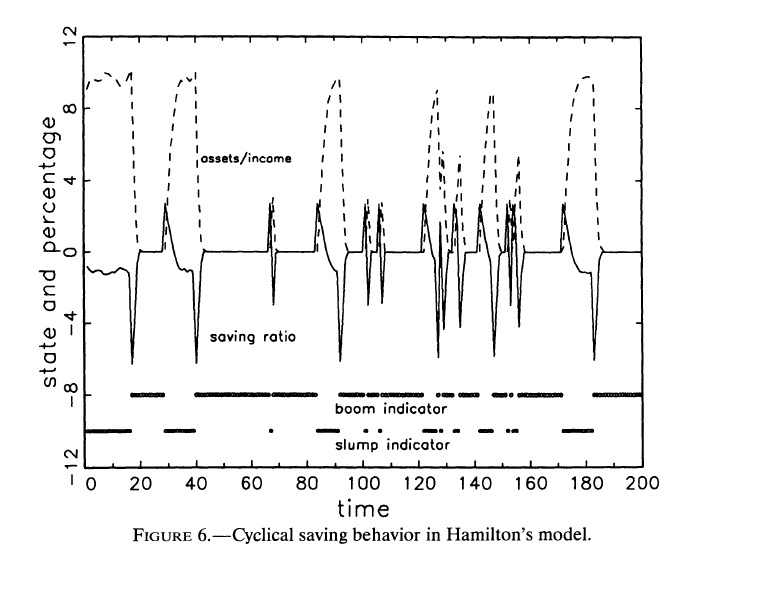
\includegraphics[height=2.5 in, scale=0.5]{figure6.jpg}
\end{figure}
\end{frame}

\begin{frame}
\frametitle{Case 5: Individual and aggregate behaviour}
\begin{itemize}
  \item Failure of the representative model does not imply BC do not behave as described here
  \item One possibility: constrained consumers, responsible for large share of consumption but only small share of savings
  \item Cont: aggregate savings accounted by unconstrained consumers
  \item Second possibility: unlikely that micro level income process mirror time-series behaviour of aggregate income
  \item Hence, start from micro data and observed income process there
\end{itemize}
\end{frame}

\begin{frame}
\frametitle{Cont.}
\begin{itemize}
  \item At the micro level, income less persistent than in the aggregate
  \item Year-to-year changes show significant negative autocorrelation, either because of measurement error or substantial transitory income in each year
  \item Start with: income process as having MA representation in first difference of logs MaCurdy(1982)
  
  \begin{equation*}
    \Delta \ln y_{t} - \mu = \epsilon_{t} + \epsilon_{t - 1}
  \end{equation*}
\end{itemize}
\end{frame}

\begin{frame}
\frametitle{Cont, 1}
\begin{itemize}
  \item MaCurdy estimates $\sigma$, the sd of $\epsilon$, the innovation to the log income process to be 0.235
  \item This would imply sd of $\Delta \ln y_{t}$ to be 0.25. In this situation agents are unlikely to borrow.
  \item Deaton assumes $\sigma$ to be between 0.10 and 0.15
\end{itemize}

Main conclusions
\begin{enumerate}
  \item Consumption functions have the general shape as before
  \item A high innovation now implies low income growth next period, so lower consumption/higher saving than before
  \item But if each income process were independent, no variation in aggregate income growth rates as savings and dissavings would cancel out in aggregate
\end{enumerate}
\end{frame}

\begin{frame}
\frametitle{Cont, 2}
Assume now that consumer receives aggregate shock with idiosyncratic component
   
  \begin{equation*}
    \Delta \ln y_{t} - g = z_{1t} + z_{2t} + z_{3t}
  \end{equation*}

where \( z_{1t} = \epsilon_{1t} + \beta \epsilon_{1t - 1}\), \( z_{2t} = \epsilon_{2t} \) and \( z_{3t} = \epsilon_{3t} +  \epsilon_{3t - 1}\) \\\

\( z_{1t}\) is common to all, others are idiosyncratic. Individual has no way of separating the three components, observes only their sum, which is IMA(1,1). Effectively implying, consumers do not observe aggregate shocks, even with a lag.
\end{frame}

\begin{frame}
\frametitle{Cont, 3}
\begin{itemize}
  \item Individual growth is negatively correlated, aggregate growth positively correlated
  \item Simulations and subsequent aggregation shows that in such a situation savings ratios are procyclical
  \item Assets, however, are always positive
  \item Model provides a means of reconciling orthogonality condition failures in the micro and macro data
\end{itemize}

\end{frame}

\begin{frame}
\frametitle{Conclusion, 1}
\begin{enumerate}
  \item i.i.d income: consumption very smooth, buffer stock behaviour strong
  \item stationary but serially correlated: consumption more noisy, buffer stock behaviour less likely
  \item random walk: limiting case, consumption = income
  \item labor shock mimics aggregate growth: counter-cyclical savings
  \item aggregate and individual combined: potential to generate savings in the aggregate, replicate data
\end{enumerate}
\end{frame}

\begin{frame}
\frametitle{Conclusion, 2}
\begin{enumerate}
  \item Story incomplete in many aspects (few financial assets, but high housing wealth and pension rights, need to integrate them into the analysis)
  \item No claim that all agents are liquidity constrained
  \item Relatively patient as well as impatient ones, the former ones likely to accumulate capital as in the standard LC model
  \item Deaton believes that such people are in minority, although they hold disproportionate share of agg. savings and wealth accumulation
  \item aggregate and individual combined: potential to generate savings in the aggregate, replicate data
\end{enumerate}
\end{frame}

\end{document} 







 
